\documentclass[]{report}
\usepackage{xeCJK}
\setCJKmainfont{Songti SC}
\setCJKsansfont{PingFang SC}

\title{Quantifying Ascorbic Acid Oxidation Kinetics in Orange Juice}
\author{John Doe}
\id{270332}
\project{Biology Experiment II}
\reportnum{8}
\date{\today}

\begin{document}
\maketitle

\begin{abstract}
抗坏血酸(维生素 C)是人类饮食中不可或缺的微量营养素,缺乏会导致坏血病等疾病。与大多数哺乳动物不同,由于进化过程中基因丢失,人类无法合成抗坏血酸,只能依靠从膳食中摄入水果和蔬菜来满足需求。本研究旨在量化橙汁在空气中的抗坏血酸氧化率。取等量鲜榨果汁,将其暴露在环境氧气中 3-25 分钟。用染料二氯苯酚靛酚(DCPIP)定时滴定剩余的抗坏血酸。结果显示,一阶衰减动力学速率为 3.443 μg/mL/min,21.1 分钟的空气暴露可保留 90\% 的初始维生素 C 水平。这些发现为最大限度地从橙汁中摄取抗坏血酸提供了预测保质期的建议。鲜榨果汁在制作完成后应尽快饮用,以免发生严重的氧化损失。
\end{abstract}

\begin{keywords}
Ascorbic Acid; Oxidation Kinetics; Orange Juice; Nutritional Quality Control
\end{keywords}

\begin{multicols}{2}
\section{Introduction}
Ascorbic acid, or vitamin C, is an essential micronutrient for humans required in the diet. Fruits like oranges are prime dietary sources. Ascorbic acid is absorbed primarily in the small intestine and transported throughout the body via the bloodstream. It is stored in various tissues, including the liver, kidneys, and adrenal glands. The current recommended dietary allowance for ascorbic acid is 90 mg/day for adult men and 75 mg/day for adult women. 

$$\chemfig[atom sep = 0.8]{HO-[:-30]-[:30](-[:90]OH)-[:-30]*5(-(-HO)=(-OH)-(=O)-O-)}$$

Vitamin C plays important roles in the human body - as a cofactor for biosynthesizing collagen, absorbing dietary iron, acting as an antioxidant, supporting immune cell function, and producing neurotransmitters. An inadequate intake can lead to lowered resistance to infections, poor wound healing, and development of scurvy disease. 

Unlike most mammals, humans lack the ability to synthesize ascorbic acid endogenously due to mutations in the gene encoding L-gulonolactone oxidase (GULO) enzyme \cite{wikipedia}. This loss of biosynthetic capacity is estimated to have occurred about 60 million years ago in ancestral primates. As a result, humans rely solely on dietary intake to meet daily ascorbic acid requirements.

The loss of ascorbic acid synthesis in humans is thought to have been a trade-off for other evolutionary advantages. Some possible explanations for the loss of GULO include:

\begin{itemize}
    \item Reduced reliance on vitamin C-rich fruits: As humans evolved a more omnivorous diet, the need to produce ascorbic acid may have diminished.
    \item Compensation by other antioxidants: Other antioxidants, such as vitamin E and glutathione, may have partially compensated for the loss of ascorbic acid synthesis.
    \item Maintenance of other metabolic pathways: The loss of GULO may have allowed for the optimization of other metabolic pathways.
\end{itemize}

Ascorbic acid is a labile compound and readily undergoes oxidation, particularly in aqueous environments and under exposure to oxygen, heat, and light. 

\begin{scheme*}
    \centering
    \scalebox{0.8}{\chemfig[atom sep = 0.8]{*5((-HO)=(-OH)-(=O)-O-(-[:150](-[:90]OH)-[:-150]-[:150]OH)-)}} + $\mathrm{O_2}$ $\rightarrow$ \scalebox{0.8}{\chemfig[atom sep = 0.8]{*5((=O)-(=O)-(=O)-O-(-[:150](-[:90]OH)-[:-150]-[:150]HO)-)}} + $\mathrm{2H^+}$ + $\mathrm{2e^-}$
    \caption{Oxidation of Ascorbic Acid}
    \label{sch:oxidation}
\end{scheme*}

Oxidation converts ascorbic acid to its oxidized form, dehydroascorbic acid, which is less biologically active \cite{messerschmidt2010}. Factors affecting ascorbic acid oxidation include:

\begin{itemize}
    \item pH: Ascorbic acid is more stable at acidic pH levels and becomes less stable as the pH increases.
    \item Temperature: Ascorbic acid degrades more rapidly at higher temperatures.
    \item Oxygen Exposure: Exposure to oxygen accelerates the oxidation of ascorbic acid.
    \item Presence of Metal Ions: Metal ions, such as copper and iron, can catalyze the oxidation of ascorbic acid.
\end{itemize}

This study aimed to determine the oxidation rate of ascorbic acid in orange juice when exposed to air. While previous research has profiled vitamin C levels in oranges \cite{vines1963}, little is known regarding kinetics of its oxidative decay over time. Elucidating this relationship can guide recommendations for optimal storage and consumption after juicing.

To achieve this objective, fresh orange juice was exposed to air for varying durations up to 25 minutes. The concentration of remaining ascorbic acid after each timed interval was titrated using the dye DCPIP, which gets reduced from blue to colorless in proportion to the vitamin C present. The rate of oxidative depletion was calculated by regression analysis.

We hypothesized that ascorbic acid degradation would follow first-order decay kinetics depending on duration of air exposure. The findings are expected to quantify the shelf life of orange juice with respect to preservation of vitamin C content. They may also allow fruit juice processors to define time limits for consumption while retaining beneficial phytonutrient levels.

\section{Methods}
\subsection{Experimental Design}
This was an in vitro observational study tracking the oxidative degradation of ascorbic acid in orange juice under ambient air exposure over time. The independent variable was duration of air exposure at room temperature. The dependent variable was concentration of remaining ascorbic acid measured by titration.

\subsection{Materials}
Fresh oranges; mortar and pestle for juicing; 0.1\% dichlorophenolindophenol (DCPIP) titrant solution; 1\% and 4.8\% oxalic acid solutions; 50 mL volumetric flask; 10 mL graduated cylinders; burette.

\subsection{Procedures}
24g oranges were juiced and filtered. The juice was made up to 50 mL in a volumetric flask as the stock solution. Six 8.33 mL samples were aliquoted into graduated cylinders and exposed to air for 3, 5, 9, 13, 17 and 25 minutes respectively. At the designated time points, 1.67 mL of 4.8\% oxalic acid was added to each sample. Within 2 minutes, the solutions were titrated with 0.1\% DCPIP till a faint pink endpoint color persisted. 

The 0.1\% DCPIP solution was standardized by titrating 1 mL of 1\% ascorbic acid standard solution diluted with 9 mL of 1\% oxalic acid. A blank titration was performed with 10 mL of 1\% oxalic acid only.

\begin{scheme*}
    \centering
    \scalebox{0.6}{\chemfig[atom sep = 0.8]{*5((-HO)=(-OH)-(=O)-O-(-[:150](-[:90]OH)-[:-150]-[:150]HO)-)}} + \scalebox{0.6}{\chemfig[atom sep = 0.8]{*6((=O)-(-Cl)=-(=N-[:-30]*6(=-=(-OH)-=-))-=(-Cl)-)}} $\rightarrow$ \scalebox{0.6}{\chemfig[atom sep = 0.8]{*5((=O)-(=O)-(=O)-O-(-[:150](-[:90]OH)-[:-150]-[:150]HO)-)}} + \scalebox{0.6}{\chemfig[atom sep = 0.8]{*6((-HO)-(-Cl)=-(-NH-[:-30]*6(=-=(-OH)-=-))=-(-Cl)=)}}
    \caption{Titration of Ascorbic Acid with DCPIP}
    \label{sch:titration}
\end{scheme*}

\subsection{Data Collection and Analysis}
The volume of DCPIP solution used up corresponding to the amount of ascorbic acid present was recorded for each sample. From the standard solution titration, the molar equivalence between DCPIP and ascorbic acid was calculated. This relation was used to determine concentration of residual ascorbic acid in the test samples. A linear regression plot of concentration over time was constructed. The slope gave the oxidation rate.

\subsection{Reliability and Validity}
The standardized DCPIP concentration ensured accuracy. Rapid quenching by oxalic acid prevented further ascorbic acid oxidation during titration. The linear range of measurements established reliability. Replicates were not feasible due to the continuous, real-time nature of oxidative decay.

\section{Results}
\subsection{Standardization and Control}
The standardization titration was performed by mixing 1 mL of 1\% ascorbic acid standard solution with 9 mL of 1\% oxalic acid, and titrating with 0.1\% DCPIP solution. It required 1.66 mL of DCPIP to reach the faint pink endpoint.

The negative control titration was carried out by titrating 10 mL of 1\% oxalic acid blank with 0.1\% DCPIP. Only 0.01 mL of DCPIP was consumed.

These results demonstrate that oxalic acid does not react with DCPIP and therefore does not interfere with the titration. Additionally, based on the volumes used, the molar equivalence was established to be that 1 mL of 0.1\% DCPIP solution corresponds to the reaction with 6.024 mg of ascorbic acid under the conditions used.

\subsection{Titration of Orange Juice Samples}
Six 8.33 mL aliquots of freshly squeezed orange juice were exposed to air for 3, 5, 9, 13, 17 and 25 minutes. To quench oxidation, 1.67 mL of 4.8\% oxalic acid was added at each pre-set interval. The samples were rapidly titrated with standardized 0.1\% DCPIP solution (Table \ref{tab:titration}).

\begin{table*}[htbp]
    \centering
    \caption{Volumes of 0.1\% DCPIP Solution Used in Titrating Orange Juice Samples}
    \label{tab:titration}
    \begin{tabularx}{\textwidth}{rcccccc}
        \toprule
        Exposure Time/min & 3 & 5 & 9 & 13 & 17 & 25 \\
        \midrule
        Volume of DCPIP/mL & 1.00 & 0.99 & 0.96 & 0.92 & 0.92 & 0.90 \\
        \(\mathrm{[AsA]}\) in Juice/$\mathrm{\mu g\cdot mL^{-1}}$ & 723.169 & 715.938 & 694.242 & 665.316 & 665.316 & 650.852 \\
        \bottomrule
    \end{tabularx}
\end{table*}

\begin{figure*}[htbp]
    \centering
    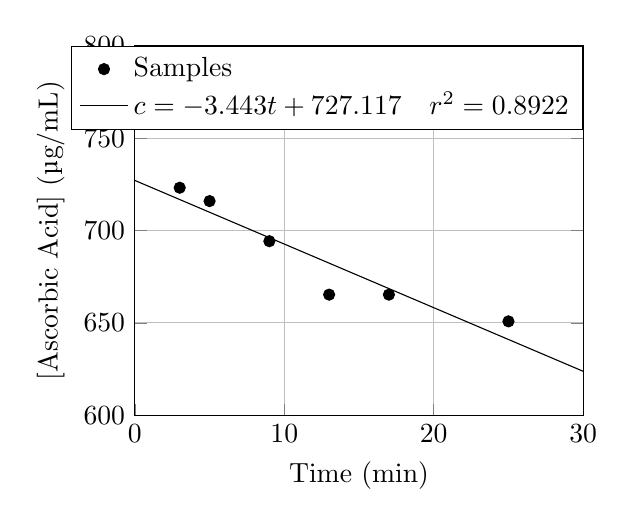
\begin{tikzpicture}
        \begin{axis}[
            xlabel={Time (min)},
            ylabel={[Ascorbic Acid] (µg/mL)},
            xmin=0, xmax=30,
            ymin=600, ymax=800,
            grid=both,
            width=0.6\textwidth,
            legend style={at={(1,1)},anchor=north east},
            legend entries={Samples, $c = -3.443 t + 727.117\quad r^2=0.8922$},
            legend cell align={left}
        ]
            \addplot[only marks,mark=*,mark size=2pt,black] table {
                3 723.169
                5 715.938
                9 694.242
                13 665.316
                17 665.316
                25 650.852
            };
            \addplot[black,domain=0:600,samples=100] {-3.443 * x + 727.117};
        \end{axis}
    \end{tikzpicture}
    \caption{Concentration of Ascorbic Acid Versus Time}
    \label{fig:regression}
\end{figure*}

The data shows a consistent downward trend in DCPIP utilization over longer air exposure periods. This indicates a steady drop in levels of oxidizable ascorbic acid as contact time elapsed. 

\subsection{Oxidation Rate Calculation}
The concentrations of residual ascorbic acid in each sample titrated were derived based on the volumes of DCPIP used and the previously determined equivalence. A linear regression plot was constructed between the concentration of ascorbic acid and exposure time to air (Figure \ref{fig:regression}).

This shows that the initial concentration of ascorbic acid in the non-exposed juice was 727.117 μg/mL. The oxidation rate was calculated as 3.443 μg/mL/min. To retain 90\% of initial ascorbic acid levels, the juice should be consumed within 21.1 mins after preparation.

Overall, the air exposure intervals resulted in a consistent decay of ascorbic acid levels in orange juice over time. The findings provide predictive and recommendation values for ingestion times to maximize vitamin C intake from freshly squeezed juice.

\section{Discussion}
The results demonstrate that ascorbic acid in orange juice degrades at a steady rate when exposed to air, with concentrations showing a consistent downward trend over time. The oxidation rate was determined to be 3.443 μg/mL/min. These kinetics align with the hypothesis that vitamin C decay would follow a first-order reaction dependent on air contact. 

Earlier analyses have also concluded that ascorbic acid oxidation rates are influenced by oxygen availability (see Introduction). However, this study specifically quantifies the impact of air exposure in orange juice. The findings are consistent with factors known to affect ascorbic acid stability, like temperature, pH, and metal ions \cite{wikipedia}. 

By establishing a shelf life limit of 21.1 minutes for consumption to retain 90\% vitamin C, this study provides practical guidance to optimize nutritional quality. The oxidation rate constant derived can help juice processors define maximum holding times before packaging. It also suggests that freshly squeezed orange juice should be consumed soon after preparation.

One limitation is that replication was difficult due to the continuous progression of oxidative degradation. More definitive conclusions may be possible with larger sample sizes in future studies. The in vitro conditions may also differ from stability in actual packaging. Testing shelf life in commercial cartons can improve applicability.  

Overall, this study achieved its aim of determining ascorbic acid oxidation kinetics in orange juice exposed to air. The findings contribute valuable quantitative insights into predicting and preserving vitamin C content. This has significance for nutritional intake, quality control, and commercial storage recommendations. Future research can explore effects of more complex storage conditions on these decay rates.
\end{multicols}

\bibliographystyle{apacite}
\bibliography{example.bib}
\end{document}
